% Made up for the tikra benchmark.
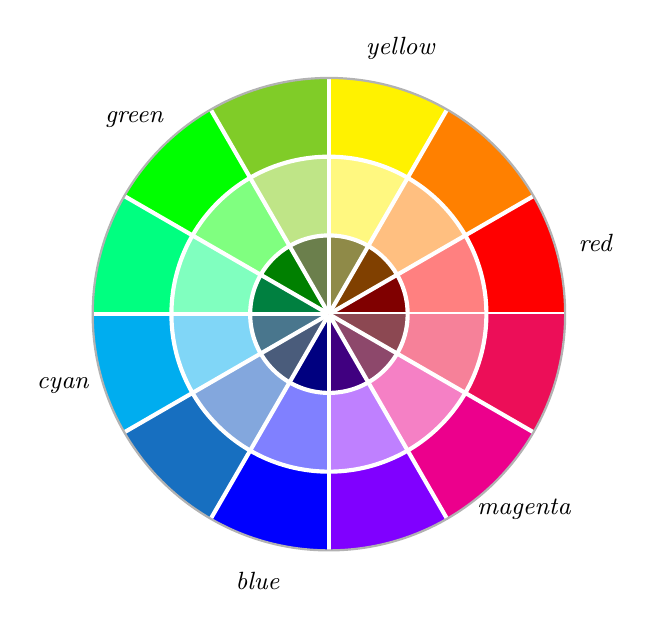
\begin{tikzpicture}
  \foreach \c [count=\i from 0] in {red, red!50!yellow, yellow, yellow!50!green, green, green!50!cyan,
      cyan, cyan!50!blue, blue, blue!50!magenta, magenta, magenta!50!red} {
    \fill[\c] (0,0) -- (\i*30:3) arc[start angle=\i*30, end angle=\i*30+30, radius=3] -- cycle;
    \fill[\c!50!white] (0,0) -- (\i*30:2) arc[start angle=\i*30, end angle=\i*30+30, radius=2] -- cycle;
    \fill[\c!50!black] (0,0) -- (\i*30:1) arc[start angle=\i*30, end angle=\i*30+30, radius=1] -- cycle;
    \draw[white, line width=1.5pt] (0,0) -- (\i*30:3);
  }
  \draw[white, line width=1.5pt] (0,0) circle (1) circle (2);
  \draw[gray!60, thick] (0,0) circle (3);
  \foreach \n/\a in {red/15, yellow/75, green/135, cyan/195, blue/255, magenta/315}
    \node[font=\small\itshape] at (\a:3.5) {\n};
\end{tikzpicture}
